\documentclass[1p]{elsarticle_modified}
%\bibliographystyle{elsarticle-num}

%\usepackage[colorlinks]{hyperref}
%\usepackage{abbrmath_seonhwa} %\Abb, \Ascr, \Acal ,\Abf, \Afrak
\usepackage{amsfonts}
\usepackage{amssymb}
\usepackage{amsmath}
\usepackage{amsthm}
\usepackage{scalefnt}
\usepackage{amsbsy}
\usepackage{kotex}
\usepackage{caption}
\usepackage{subfig}
\usepackage{color}
\usepackage{graphicx}
\usepackage{xcolor} %% white, black, red, green, blue, cyan, magenta, yellow
\usepackage{float}
\usepackage{setspace}
\usepackage{hyperref}

\usepackage{tikz}
\usetikzlibrary{arrows}

\usepackage{multirow}
\usepackage{array} % fixed length table
\usepackage{hhline}

%%%%%%%%%%%%%%%%%%%%%
\makeatletter
\renewcommand*\env@matrix[1][\arraystretch]{%
	\edef\arraystretch{#1}%
	\hskip -\arraycolsep
	\let\@ifnextchar\new@ifnextchar
	\array{*\c@MaxMatrixCols c}}
\makeatother %https://tex.stackexchange.com/questions/14071/how-can-i-increase-the-line-spacing-in-a-matrix
%%%%%%%%%%%%%%%

\usepackage[normalem]{ulem}

\newcommand{\msout}[1]{\ifmmode\text{\sout{\ensuremath{#1}}}\else\sout{#1}\fi}
%SOURCE: \msout is \stkout macro in https://tex.stackexchange.com/questions/20609/strikeout-in-math-mode

\newcommand{\cancel}[1]{
	\ifmmode
	{\color{red}\msout{#1}}
	\else
	{\color{red}\sout{#1}}
	\fi
}

\newcommand{\add}[1]{
	{\color{blue}\uwave{#1}}
}

\newcommand{\replace}[2]{
	\ifmmode
	{\color{red}\msout{#1}}{\color{blue}\uwave{#2}}
	\else
	{\color{red}\sout{#1}}{\color{blue}\uwave{#2}}
	\fi
}

\newcommand{\Sol}{\mathcal{S}} %segment
\newcommand{\D}{D} %diagram
\newcommand{\A}{\mathcal{A}} %arc


%%%%%%%%%%%%%%%%%%%%%%%%%%%%%5 test

\def\sl{\operatorname{\textup{SL}}(2,\Cbb)}
\def\psl{\operatorname{\textup{PSL}}(2,\Cbb)}
\def\quan{\mkern 1mu \triangleright \mkern 1mu}

\theoremstyle{definition}
\newtheorem{thm}{Theorem}[section]
\newtheorem{prop}[thm]{Proposition}
\newtheorem{lem}[thm]{Lemma}
\newtheorem{ques}[thm]{Question}
\newtheorem{cor}[thm]{Corollary}
\newtheorem{defn}[thm]{Definition}
\newtheorem{exam}[thm]{Example}
\newtheorem{rmk}[thm]{Remark}
\newtheorem{alg}[thm]{Algorithm}

\newcommand{\I}{\sqrt{-1}}
\begin{document}

%\begin{frontmatter}
%
%\title{Boundary parabolic representations of knots up to 8 crossings}
%
%%% Group authors per affiliation:
%\author{Yunhi Cho} 
%\address{Department of Mathematics, University of Seoul, Seoul, Korea}
%\ead{yhcho@uos.ac.kr}
%
%
%\author{Seonhwa Kim} %\fnref{s_kim}}
%\address{Center for Geometry and Physics, Institute for Basic Science, Pohang, 37673, Korea}
%\ead{ryeona17@ibs.re.kr}
%
%\author{Hyuk Kim}
%\address{Department of Mathematical Sciences, Seoul National University, Seoul 08826, Korea}
%\ead{hyukkim@snu.ac.kr}
%
%\author{Seokbeom Yoon}
%\address{Department of Mathematical Sciences, Seoul National University, Seoul, 08826,  Korea}
%\ead{sbyoon15@snu.ac.kr}
%
%\begin{abstract}
%We find all boundary parabolic representation of knots up to 8 crossings.
%
%\end{abstract}
%\begin{keyword}
%    \MSC[2010] 57M25 
%\end{keyword}
%
%\end{frontmatter}

%\linenumbers
%\tableofcontents
%
\newcommand\colored[1]{\textcolor{white}{\rule[-0.35ex]{0.8em}{1.4ex}}\kern-0.8em\color{red} #1}%
%\newcommand\colored[1]{\textcolor{white}{ #1}\kern-2.17ex	\textcolor{white}{ #1}\kern-1.81ex	\textcolor{white}{ #1}\kern-2.15ex\color{red}#1	}

{\Large $\underline{11a_{107}~(K11a_{107})}$}

\setlength{\tabcolsep}{10pt}
\renewcommand{\arraystretch}{1.6}
\vspace{1cm}\begin{tabular}{m{100pt}>{\centering\arraybackslash}m{274pt}}
\multirow{5}{120pt}{
	\centering
	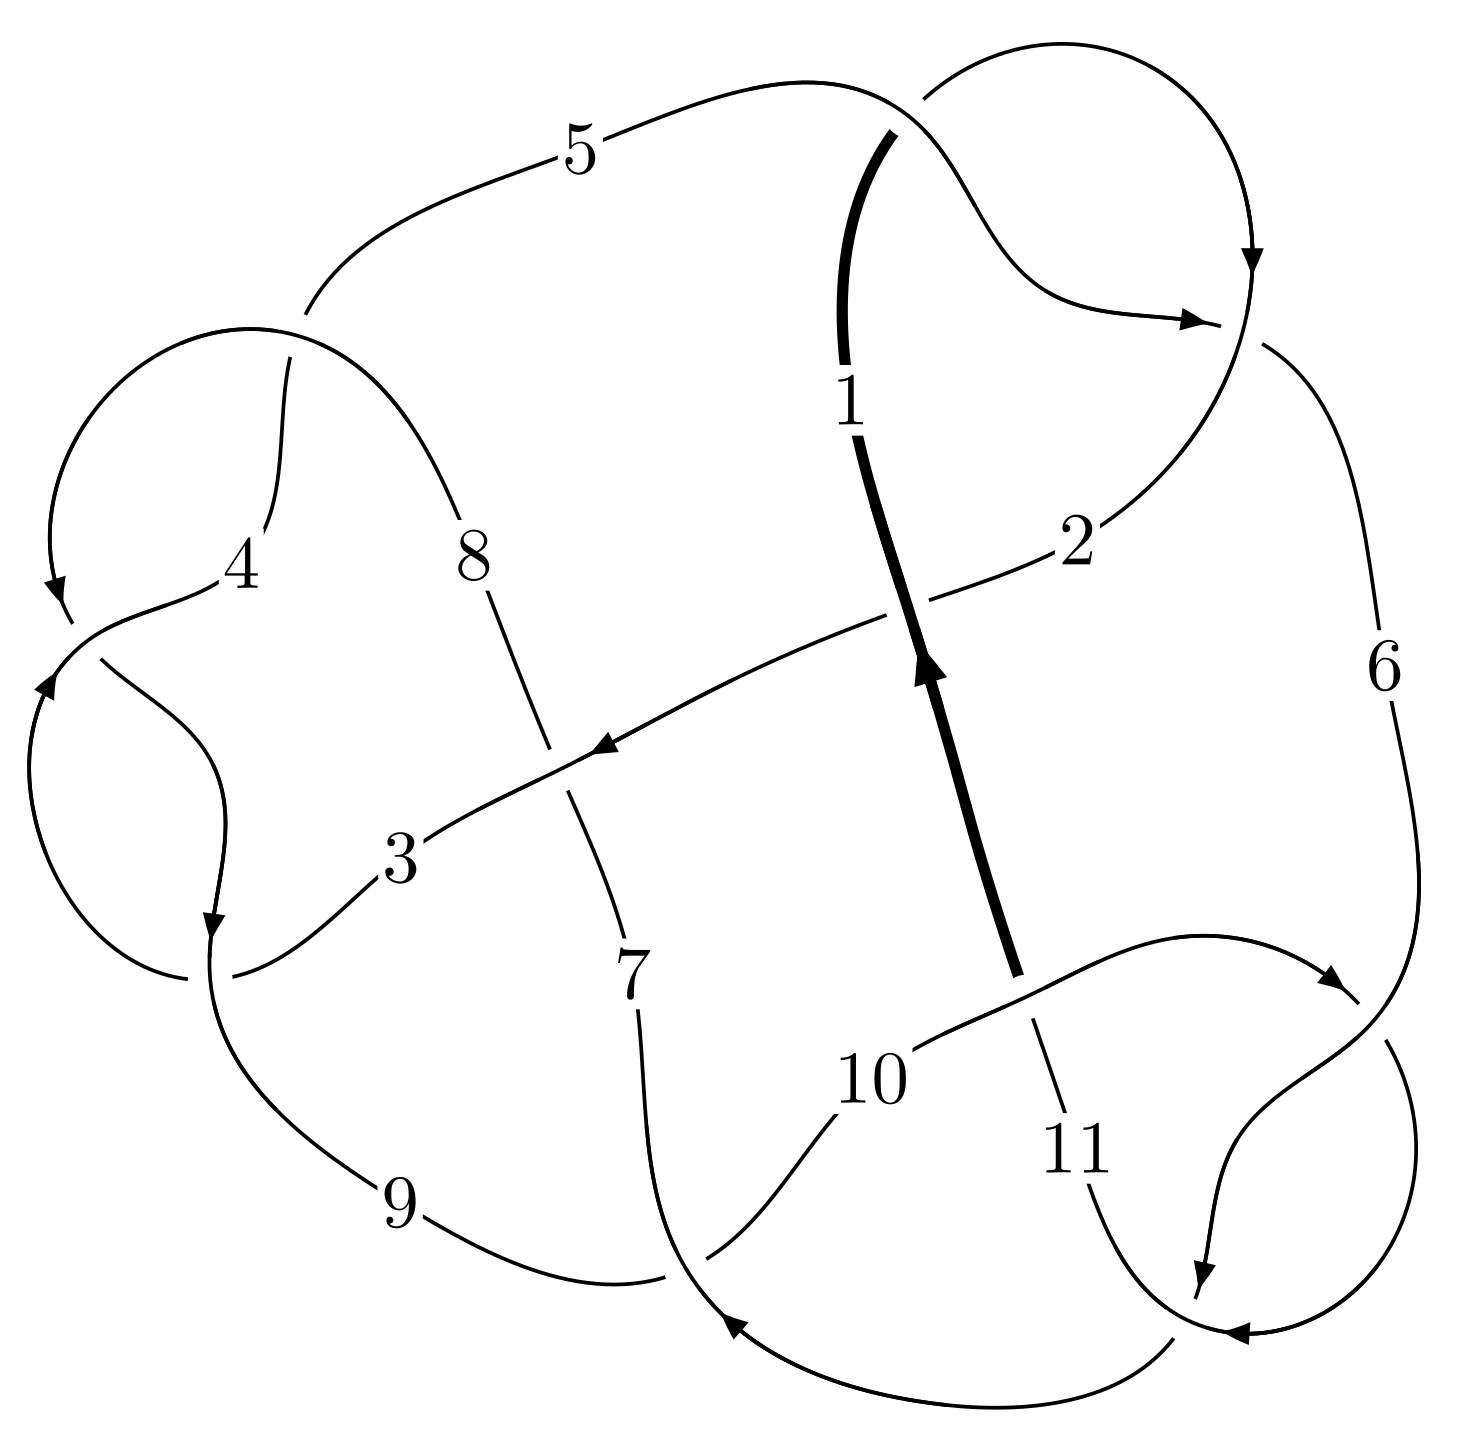
\includegraphics[width=112pt]{../../../GIT/diagram.site/Diagrams/png/356_11a_107.png}\\
\ \ \ A knot diagram\footnotemark}&
\allowdisplaybreaks
\textbf{Linearized knot diagam} \\
\cline{2-2}
 &
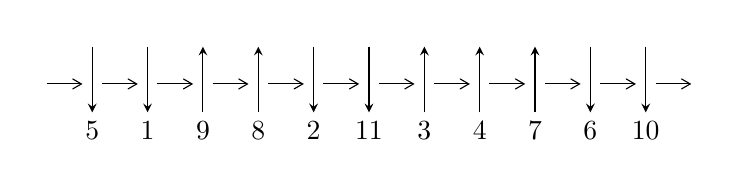
\begin{tikzpicture}[x=20pt, y=17pt]
	% nodes
	\node (C0) at (0, 0) {};
	\node (C1) at (1, 0) {};
	\node (C1U) at (1, +1) {};
	\node (C1D) at (1, -1) {5};

	\node (C2) at (2, 0) {};
	\node (C2U) at (2, +1) {};
	\node (C2D) at (2, -1) {1};

	\node (C3) at (3, 0) {};
	\node (C3U) at (3, +1) {};
	\node (C3D) at (3, -1) {9};

	\node (C4) at (4, 0) {};
	\node (C4U) at (4, +1) {};
	\node (C4D) at (4, -1) {8};

	\node (C5) at (5, 0) {};
	\node (C5U) at (5, +1) {};
	\node (C5D) at (5, -1) {2};

	\node (C6) at (6, 0) {};
	\node (C6U) at (6, +1) {};
	\node (C6D) at (6, -1) {11};

	\node (C7) at (7, 0) {};
	\node (C7U) at (7, +1) {};
	\node (C7D) at (7, -1) {3};

	\node (C8) at (8, 0) {};
	\node (C8U) at (8, +1) {};
	\node (C8D) at (8, -1) {4};

	\node (C9) at (9, 0) {};
	\node (C9U) at (9, +1) {};
	\node (C9D) at (9, -1) {7};

	\node (C10) at (10, 0) {};
	\node (C10U) at (10, +1) {};
	\node (C10D) at (10, -1) {6};

	\node (C11) at (11, 0) {};
	\node (C11U) at (11, +1) {};
	\node (C11D) at (11, -1) {10};
	\node (C12) at (12, 0) {};

	% arrows
	\draw[->,>={angle 60}]
	(C0) edge (C1) (C1) edge (C2) (C2) edge (C3) (C3) edge (C4) (C4) edge (C5) (C5) edge (C6) (C6) edge (C7) (C7) edge (C8) (C8) edge (C9) (C9) edge (C10) (C10) edge (C11) (C11) edge (C12) ;	\draw[->,>=stealth]
	(C1U) edge (C1D) (C2U) edge (C2D) (C3D) edge (C3U) (C4D) edge (C4U) (C5U) edge (C5D) (C6U) edge (C6D) (C7D) edge (C7U) (C8D) edge (C8U) (C9D) edge (C9U) (C10U) edge (C10D) (C11U) edge (C11D) ;
	\end{tikzpicture} \\
\hhline{~~} \\& 
\textbf{Solving Sequence} \\ \cline{2-2} 
 &
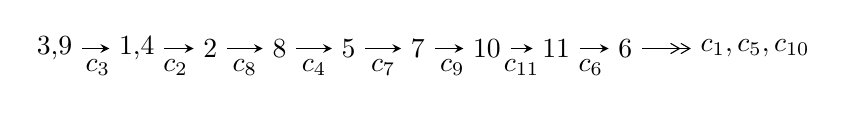
\begin{tikzpicture}[x=25pt, y=7pt]
	% node
	\node (A0) at (-1/8, 0) {3,9};
	\node (A1) at (17/16, 0) {1,4};
	\node (A2) at (17/8, 0) {2};
	\node (A3) at (25/8, 0) {8};
	\node (A4) at (33/8, 0) {5};
	\node (A5) at (41/8, 0) {7};
	\node (A6) at (49/8, 0) {10};
	\node (A7) at (57/8, 0) {11};
	\node (A8) at (65/8, 0) {6};
	\node (C1) at (1/2, -1) {$c_{3}$};
	\node (C2) at (13/8, -1) {$c_{2}$};
	\node (C3) at (21/8, -1) {$c_{8}$};
	\node (C4) at (29/8, -1) {$c_{4}$};
	\node (C5) at (37/8, -1) {$c_{7}$};
	\node (C6) at (45/8, -1) {$c_{9}$};
	\node (C7) at (53/8, -1) {$c_{11}$};
	\node (C8) at (61/8, -1) {$c_{6}$};
	\node (A9) at (10, 0) {$c_{1},c_{5},c_{10}$};

	% edge
	\draw[->,>=stealth]	
	(A0) edge (A1) (A1) edge (A2) (A2) edge (A3) (A3) edge (A4) (A4) edge (A5) (A5) edge (A6) (A6) edge (A7) (A7) edge (A8) ;
	\draw[->>,>={angle 60}]	
	(A8) edge (A9);
\end{tikzpicture} \\ 

\end{tabular} \\

\footnotetext{
The image of knot diagram is generated by the software ``\textbf{Draw programme}" developed by Andrew Bartholomew(\url{http://www.layer8.co.uk/maths/draw/index.htm\#Running-draw}), where we modified some parts for our purpose(\url{https://github.com/CATsTAILs/LinksPainter}).
}\phantom \\ \newline 
\centering \textbf{Ideals for irreducible components\footnotemark of $X_{\text{par}}$} 
 
\begin{align*}
I^u_{1}&=\langle 
- u^{21}-2 u^{20}+\cdots+b-1,\;- u^{21}-3 u^{20}+\cdots+2 a-4,\;u^{22}+3 u^{21}+\cdots+8 u+2\rangle \\
I^u_{2}&=\langle 
-18 u^{17} a+8 u^{17}+\cdots-23 a+44,\;-2 u^{17} a+2 u^{17}+\cdots-6 a+5,\;u^{18}- u^{17}+\cdots+3 u-1\rangle \\
I^u_{3}&=\langle 
b+1,\;2 a- u,\;u^2+2\rangle \\
\\
I^v_{1}&=\langle 
a,\;b+1,\;v+1\rangle \\
\end{align*}
\raggedright * 4 irreducible components of $\dim_{\mathbb{C}}=0$, with total 61 representations.\\
\footnotetext{All coefficients of polynomials are rational numbers. But the coefficients are sometimes approximated in decimal forms when there is not enough margin.}
\newpage
\renewcommand{\arraystretch}{1}
\centering \section*{I. $I^u_{1}= \langle - u^{21}-2 u^{20}+\cdots+b-1,\;- u^{21}-3 u^{20}+\cdots+2 a-4,\;u^{22}+3 u^{21}+\cdots+8 u+2 \rangle$}
\flushleft \textbf{(i) Arc colorings}\\
\begin{tabular}{m{7pt} m{180pt} m{7pt} m{180pt} }
\flushright $a_{3}=$&$\begin{pmatrix}1\\0\end{pmatrix}$ \\
\flushright $a_{9}=$&$\begin{pmatrix}0\\u\end{pmatrix}$ \\
\flushright $a_{1}=$&$\begin{pmatrix}\frac{1}{2} u^{21}+\frac{3}{2} u^{20}+\cdots+3 u+2\\u^{21}+2 u^{20}+\cdots+4 u+1\end{pmatrix}$ \\
\flushright $a_{4}=$&$\begin{pmatrix}1\\- u^2\end{pmatrix}$ \\
\flushright $a_{2}=$&$\begin{pmatrix}\frac{1}{2} u^{21}+\frac{1}{2} u^{20}+\cdots+u+1\\- u^{21}-2 u^{20}+\cdots-4 u-1\end{pmatrix}$ \\
\flushright $a_{8}=$&$\begin{pmatrix}- u\\u^3+u\end{pmatrix}$ \\
\flushright $a_{5}=$&$\begin{pmatrix}u^2+1\\- u^4-2 u^2\end{pmatrix}$ \\
\flushright $a_{7}=$&$\begin{pmatrix}- u^3-2 u\\u^3+u\end{pmatrix}$ \\
\flushright $a_{10}=$&$\begin{pmatrix}u^7+4 u^5+4 u^3\\- u^7-3 u^5-2 u^3+u\end{pmatrix}$ \\
\flushright $a_{11}=$&$\begin{pmatrix}-\frac{1}{2} u^{21}-\frac{1}{2} u^{20}+\cdots-3 u^2- u\\u^{21}+2 u^{20}+\cdots+3 u+1\end{pmatrix}$ \\
\flushright $a_{6}=$&$\begin{pmatrix}\frac{3}{2} u^{21}+\frac{9}{2} u^{20}+\cdots+16 u+6\\- u^{19}-3 u^{18}+\cdots-6 u-3\end{pmatrix}$\\ \flushright $a_{6}=$&$\begin{pmatrix}\frac{3}{2} u^{21}+\frac{9}{2} u^{20}+\cdots+16 u+6\\- u^{19}-3 u^{18}+\cdots-6 u-3\end{pmatrix}$\\&\end{tabular}
\flushleft \textbf{(ii) Obstruction class $= -1$}\\~\\
\flushleft \textbf{(iii) Cusp Shapes $= 8 u^{21}+18 u^{20}+102 u^{19}+188 u^{18}+534 u^{17}+810 u^{16}+1478 u^{15}+1814 u^{14}+2262 u^{13}+2108 u^{12}+1682 u^{11}+880 u^{10}+82 u^9-518 u^8-676 u^7-544 u^6-244 u^5+10 u^4+118 u^3+108 u^2+62 u+20$}\\~\\
\newpage\renewcommand{\arraystretch}{1}
\flushleft \textbf{(iv) u-Polynomials at the component}\newline \\
\begin{tabular}{m{50pt}|m{274pt}}
Crossings & \hspace{64pt}u-Polynomials at each crossing \\
\hline $$\begin{aligned}c_{1},c_{5},c_{6}\\c_{10}\end{aligned}$$&$\begin{aligned}
&u^{22}+u^{21}+\cdots+u+1
\end{aligned}$\\
\hline $$\begin{aligned}c_{2},c_{11}\end{aligned}$$&$\begin{aligned}
&u^{22}+11 u^{21}+\cdots+3 u+1
\end{aligned}$\\
\hline $$\begin{aligned}c_{3},c_{4},c_{8}\end{aligned}$$&$\begin{aligned}
&u^{22}-3 u^{21}+\cdots-8 u+2
\end{aligned}$\\
\hline $$\begin{aligned}c_{7}\end{aligned}$$&$\begin{aligned}
&u^{22}+3 u^{21}+\cdots-16 u+2
\end{aligned}$\\
\hline $$\begin{aligned}c_{9}\end{aligned}$$&$\begin{aligned}
&u^{22}+3 u^{21}+\cdots-64 u^2+16
\end{aligned}$\\
\hline
\end{tabular}\\~\\
\newpage\renewcommand{\arraystretch}{1}
\flushleft \textbf{(v) Riley Polynomials at the component}\newline \\
\begin{tabular}{m{50pt}|m{274pt}}
Crossings & \hspace{64pt}Riley Polynomials at each crossing \\
\hline $$\begin{aligned}c_{1},c_{5},c_{6}\\c_{10}\end{aligned}$$&$\begin{aligned}
&y^{22}-11 y^{21}+\cdots-3 y+1
\end{aligned}$\\
\hline $$\begin{aligned}c_{2},c_{11}\end{aligned}$$&$\begin{aligned}
&y^{22}+5 y^{21}+\cdots+5 y+1
\end{aligned}$\\
\hline $$\begin{aligned}c_{3},c_{4},c_{8}\end{aligned}$$&$\begin{aligned}
&y^{22}+21 y^{21}+\cdots+8 y+4
\end{aligned}$\\
\hline $$\begin{aligned}c_{7}\end{aligned}$$&$\begin{aligned}
&y^{22}+9 y^{21}+\cdots-24 y+4
\end{aligned}$\\
\hline $$\begin{aligned}c_{9}\end{aligned}$$&$\begin{aligned}
&y^{22}+13 y^{21}+\cdots-2048 y+256
\end{aligned}$\\
\hline
\end{tabular}\\~\\
\newpage\flushleft \textbf{(vi) Complex Volumes and Cusp Shapes}
$$\begin{array}{c|c|c}  
\text{Solutions to }I^u_{1}& \I (\text{vol} + \sqrt{-1}CS) & \text{Cusp shape}\\
 \hline 
\begin{aligned}
u &= \phantom{-}0.099141 + 1.060720 I \\
a &= \phantom{-}0.817278 + 0.592678 I \\
b &= -0.080492 - 0.751236 I\end{aligned}
 & -0.63227 - 1.36325 I & -0.37432 + 3.42755 I \\ \hline\begin{aligned}
u &= \phantom{-}0.099141 - 1.060720 I \\
a &= \phantom{-}0.817278 - 0.592678 I \\
b &= -0.080492 + 0.751236 I\end{aligned}
 & -0.63227 + 1.36325 I & -0.37432 - 3.42755 I \\ \hline\begin{aligned}
u &= -0.586314 + 0.582688 I \\
a &= \phantom{-}1.103980 - 0.244349 I \\
b &= -1.09402 + 1.14571 I\end{aligned}
 & -5.03371 + 6.28370 I & -5.65704 - 3.70414 I \\ \hline\begin{aligned}
u &= -0.586314 - 0.582688 I \\
a &= \phantom{-}1.103980 + 0.244349 I \\
b &= -1.09402 - 1.14571 I\end{aligned}
 & -5.03371 - 6.28370 I & -5.65704 + 3.70414 I \\ \hline\begin{aligned}
u &= -0.721391 + 0.399058 I \\
a &= -0.26176 + 2.28725 I \\
b &= -1.12690 - 1.26320 I\end{aligned}
 & -4.37280 - 10.68880 I & -4.26664 + 8.95764 I \\ \hline\begin{aligned}
u &= -0.721391 - 0.399058 I \\
a &= -0.26176 - 2.28725 I \\
b &= -1.12690 + 1.26320 I\end{aligned}
 & -4.37280 + 10.68880 I & -4.26664 - 8.95764 I \\ \hline\begin{aligned}
u &= \phantom{-}0.689708 + 0.121552 I \\
a &= \phantom{-}0.53466 - 2.02230 I \\
b &= -0.385181 + 0.996181 I\end{aligned}
 & \phantom{-}2.02679 + 4.63959 I & \phantom{-}2.23017 - 7.26462 I \\ \hline\begin{aligned}
u &= \phantom{-}0.689708 - 0.121552 I \\
a &= \phantom{-}0.53466 + 2.02230 I \\
b &= -0.385181 - 0.996181 I\end{aligned}
 & \phantom{-}2.02679 - 4.63959 I & \phantom{-}2.23017 + 7.26462 I \\ \hline\begin{aligned}
u &= -0.008426 + 0.680012 I \\
a &= \phantom{-}0.709637 + 0.189298 I \\
b &= -0.205333 - 0.521077 I\end{aligned}
 & -0.56996 - 1.46936 I & -1.98240 + 4.73317 I \\ \hline\begin{aligned}
u &= -0.008426 - 0.680012 I \\
a &= \phantom{-}0.709637 - 0.189298 I \\
b &= -0.205333 + 0.521077 I\end{aligned}
 & -0.56996 + 1.46936 I & -1.98240 - 4.73317 I\\
 \hline 
 \end{array}$$\newpage$$\begin{array}{c|c|c}  
\text{Solutions to }I^u_{1}& \I (\text{vol} + \sqrt{-1}CS) & \text{Cusp shape}\\
 \hline 
\begin{aligned}
u &= \phantom{-}0.266288 + 1.293670 I \\
a &= -0.431973 - 1.182530 I \\
b &= -0.556035 + 1.146260 I\end{aligned}
 & -2.37652 + 8.11206 I & -3.44648 - 8.70000 I \\ \hline\begin{aligned}
u &= \phantom{-}0.266288 - 1.293670 I \\
a &= -0.431973 + 1.182530 I \\
b &= -0.556035 - 1.146260 I\end{aligned}
 & -2.37652 - 8.11206 I & -3.44648 + 8.70000 I \\ \hline\begin{aligned}
u &= -0.594447 + 0.259956 I \\
a &= \phantom{-}0.630368 - 0.825820 I \\
b &= \phantom{-}0.355452 + 0.329277 I\end{aligned}
 & \phantom{-}1.11971 - 1.23902 I & \phantom{-}3.65819 + 2.25067 I \\ \hline\begin{aligned}
u &= -0.594447 - 0.259956 I \\
a &= \phantom{-}0.630368 + 0.825820 I \\
b &= \phantom{-}0.355452 - 0.329277 I\end{aligned}
 & \phantom{-}1.11971 + 1.23902 I & \phantom{-}3.65819 - 2.25067 I \\ \hline\begin{aligned}
u &= -0.22843 + 1.41110 I \\
a &= \phantom{-}0.951917 - 0.568853 I \\
b &= \phantom{-}0.595163 + 0.296817 I\end{aligned}
 & -4.25973 - 4.25337 I & -1.79063 + 2.48164 I \\ \hline\begin{aligned}
u &= -0.22843 - 1.41110 I \\
a &= \phantom{-}0.951917 + 0.568853 I \\
b &= \phantom{-}0.595163 - 0.296817 I\end{aligned}
 & -4.25973 + 4.25337 I & -1.79063 - 2.48164 I \\ \hline\begin{aligned}
u &= \phantom{-}0.03042 + 1.47870 I \\
a &= \phantom{-}0.268624 - 0.247145 I \\
b &= -0.614464 - 0.368195 I\end{aligned}
 & -7.27839 - 1.13244 I & -4.78640 + 6.09747 I \\ \hline\begin{aligned}
u &= \phantom{-}0.03042 - 1.47870 I \\
a &= \phantom{-}0.268624 + 0.247145 I \\
b &= -0.614464 + 0.368195 I\end{aligned}
 & -7.27839 + 1.13244 I & -4.78640 - 6.09747 I \\ \hline\begin{aligned}
u &= -0.27059 + 1.46672 I \\
a &= -1.36291 + 1.22986 I \\
b &= -1.19776 - 1.31540 I\end{aligned}
 & -10.3818 - 14.3064 I & -7.97941 + 8.76372 I \\ \hline\begin{aligned}
u &= -0.27059 - 1.46672 I \\
a &= -1.36291 - 1.22986 I \\
b &= -1.19776 + 1.31540 I\end{aligned}
 & -10.3818 + 14.3064 I & -7.97941 - 8.76372 I\\
 \hline 
 \end{array}$$\newpage$$\begin{array}{c|c|c}  
\text{Solutions to }I^u_{1}& \I (\text{vol} + \sqrt{-1}CS) & \text{Cusp shape}\\
 \hline 
\begin{aligned}
u &= -0.17596 + 1.50335 I \\
a &= \phantom{-}0.040171 + 0.648478 I \\
b &= -1.19043 + 1.03440 I\end{aligned}
 & -11.83210 + 3.58162 I & -9.60503 - 4.09544 I \\ \hline\begin{aligned}
u &= -0.17596 - 1.50335 I \\
a &= \phantom{-}0.040171 - 0.648478 I \\
b &= -1.19043 - 1.03440 I\end{aligned}
 & -11.83210 - 3.58162 I & -9.60503 + 4.09544 I\\
 \hline 
 \end{array}$$\newpage\newpage\renewcommand{\arraystretch}{1}
\centering \section*{II. $I^u_{2}= \langle -18 u^{17} a+8 u^{17}+\cdots-23 a+44,\;-2 u^{17} a+2 u^{17}+\cdots-6 a+5,\;u^{18}- u^{17}+\cdots+3 u-1 \rangle$}
\flushleft \textbf{(i) Arc colorings}\\
\begin{tabular}{m{7pt} m{180pt} m{7pt} m{180pt} }
\flushright $a_{3}=$&$\begin{pmatrix}1\\0\end{pmatrix}$ \\
\flushright $a_{9}=$&$\begin{pmatrix}0\\u\end{pmatrix}$ \\
\flushright $a_{1}=$&$\begin{pmatrix}a\\0.947368 a u^{17}-0.421053 u^{17}+\cdots+1.21053 a-2.31579\end{pmatrix}$ \\
\flushright $a_{4}=$&$\begin{pmatrix}1\\- u^2\end{pmatrix}$ \\
\flushright $a_{2}=$&$\begin{pmatrix}-0.421053 a u^{17}+0.631579 u^{17}+\cdots-0.315789 a+2.47368\\0.263158 a u^{17}+0.105263 u^{17}+\cdots+0.947368 a-2.42105\end{pmatrix}$ \\
\flushright $a_{8}=$&$\begin{pmatrix}- u\\u^3+u\end{pmatrix}$ \\
\flushright $a_{5}=$&$\begin{pmatrix}u^2+1\\- u^4-2 u^2\end{pmatrix}$ \\
\flushright $a_{7}=$&$\begin{pmatrix}- u^3-2 u\\u^3+u\end{pmatrix}$ \\
\flushright $a_{10}=$&$\begin{pmatrix}u^7+4 u^5+4 u^3\\- u^7-3 u^5-2 u^3+u\end{pmatrix}$ \\
\flushright $a_{11}=$&$\begin{pmatrix}0.947368 a u^{17}-0.421053 u^{17}+\cdots+2.21053 a-1.31579\\0.105263 a u^{17}-0.157895 u^{17}+\cdots-0.421053 a-1.36842\end{pmatrix}$ \\
\flushright $a_{6}=$&$\begin{pmatrix}1.57895 a u^{17}-1.36842 u^{17}+\cdots+3.68421 a-4.52632\\-0.105263 a u^{17}+1.15789 u^{17}+\cdots-1.57895 a+2.36842\end{pmatrix}$\\ \flushright $a_{6}=$&$\begin{pmatrix}1.57895 a u^{17}-1.36842 u^{17}+\cdots+3.68421 a-4.52632\\-0.105263 a u^{17}+1.15789 u^{17}+\cdots-1.57895 a+2.36842\end{pmatrix}$\\&\end{tabular}
\flushleft \textbf{(ii) Obstruction class $= -1$}\\~\\
\flushleft \textbf{(iii) Cusp Shapes $= 4 u^{17}-4 u^{16}+36 u^{15}-28 u^{14}+124 u^{13}-72 u^{12}+196 u^{11}-72 u^{10}+120 u^9-8 u^7+36 u^6-8 u^5+4 u^4+16 u^3-8 u+6$}\\~\\
\newpage\renewcommand{\arraystretch}{1}
\flushleft \textbf{(iv) u-Polynomials at the component}\newline \\
\begin{tabular}{m{50pt}|m{274pt}}
Crossings & \hspace{64pt}u-Polynomials at each crossing \\
\hline $$\begin{aligned}c_{1},c_{5},c_{6}\\c_{10}\end{aligned}$$&$\begin{aligned}
&u^{36}+u^{35}+\cdots-6 u-3
\end{aligned}$\\
\hline $$\begin{aligned}c_{2},c_{11}\end{aligned}$$&$\begin{aligned}
&u^{36}+21 u^{35}+\cdots+12 u+9
\end{aligned}$\\
\hline $$\begin{aligned}c_{3},c_{4},c_{8}\end{aligned}$$&$\begin{aligned}
&(u^{18}+u^{17}+\cdots-3 u-1)^{2}
\end{aligned}$\\
\hline $$\begin{aligned}c_{7}\end{aligned}$$&$\begin{aligned}
&(u^{18}- u^{17}+\cdots-13 u-5)^{2}
\end{aligned}$\\
\hline $$\begin{aligned}c_{9}\end{aligned}$$&$\begin{aligned}
&(u^{18}+3 u^{17}+\cdots+3 u+3)^{2}
\end{aligned}$\\
\hline
\end{tabular}\\~\\
\newpage\renewcommand{\arraystretch}{1}
\flushleft \textbf{(v) Riley Polynomials at the component}\newline \\
\begin{tabular}{m{50pt}|m{274pt}}
Crossings & \hspace{64pt}Riley Polynomials at each crossing \\
\hline $$\begin{aligned}c_{1},c_{5},c_{6}\\c_{10}\end{aligned}$$&$\begin{aligned}
&y^{36}-21 y^{35}+\cdots-12 y+9
\end{aligned}$\\
\hline $$\begin{aligned}c_{2},c_{11}\end{aligned}$$&$\begin{aligned}
&y^{36}-13 y^{35}+\cdots-1260 y+81
\end{aligned}$\\
\hline $$\begin{aligned}c_{3},c_{4},c_{8}\end{aligned}$$&$\begin{aligned}
&(y^{18}+17 y^{17}+\cdots-7 y+1)^{2}
\end{aligned}$\\
\hline $$\begin{aligned}c_{7}\end{aligned}$$&$\begin{aligned}
&(y^{18}+5 y^{17}+\cdots-39 y+25)^{2}
\end{aligned}$\\
\hline $$\begin{aligned}c_{9}\end{aligned}$$&$\begin{aligned}
&(y^{18}+13 y^{17}+\cdots-75 y+9)^{2}
\end{aligned}$\\
\hline
\end{tabular}\\~\\
\newpage\flushleft \textbf{(vi) Complex Volumes and Cusp Shapes}
$$\begin{array}{c|c|c}  
\text{Solutions to }I^u_{2}& \I (\text{vol} + \sqrt{-1}CS) & \text{Cusp shape}\\
 \hline 
\begin{aligned}
u &= -0.215059 + 1.214380 I \\
a &= \phantom{-}0.002300 + 1.089580 I \\
b &= -0.368793 - 0.969057 I\end{aligned}
 & -1.13659 - 3.22673 I & -0.94474 + 3.62956 I \\ \hline\begin{aligned}
u &= -0.215059 + 1.214380 I \\
a &= \phantom{-}0.975063 - 0.588954 I \\
b &= \phantom{-}0.192944 + 0.699186 I\end{aligned}
 & -1.13659 - 3.22673 I & -0.94474 + 3.62956 I \\ \hline\begin{aligned}
u &= -0.215059 - 1.214380 I \\
a &= \phantom{-}0.002300 - 1.089580 I \\
b &= -0.368793 + 0.969057 I\end{aligned}
 & -1.13659 + 3.22673 I & -0.94474 - 3.62956 I \\ \hline\begin{aligned}
u &= -0.215059 - 1.214380 I \\
a &= \phantom{-}0.975063 + 0.588954 I \\
b &= \phantom{-}0.192944 - 0.699186 I\end{aligned}
 & -1.13659 + 3.22673 I & -0.94474 - 3.62956 I \\ \hline\begin{aligned}
u &= \phantom{-}0.678984 + 0.355286 I \\
a &= \phantom{-}0.373118 + 0.790875 I \\
b &= \phantom{-}0.638489 - 0.301741 I\end{aligned}
 & -1.40107 + 5.71427 I & -0.93404 - 6.05983 I \\ \hline\begin{aligned}
u &= \phantom{-}0.678984 + 0.355286 I \\
a &= -0.15211 - 2.42083 I \\
b &= -1.01877 + 1.13385 I\end{aligned}
 & -1.40107 + 5.71427 I & -0.93404 - 6.05983 I \\ \hline\begin{aligned}
u &= \phantom{-}0.678984 - 0.355286 I \\
a &= \phantom{-}0.373118 - 0.790875 I \\
b &= \phantom{-}0.638489 + 0.301741 I\end{aligned}
 & -1.40107 - 5.71427 I & -0.93404 + 6.05983 I \\ \hline\begin{aligned}
u &= \phantom{-}0.678984 - 0.355286 I \\
a &= -0.15211 + 2.42083 I \\
b &= -1.01877 - 1.13385 I\end{aligned}
 & -1.40107 - 5.71427 I & -0.93404 + 6.05983 I \\ \hline\begin{aligned}
u &= -0.590027 + 0.406016 I \\
a &= \phantom{-}1.118520 - 0.162715 I \\
b &= -1.37030 + 0.82721 I\end{aligned}
 & -5.71606 - 1.88569 I & -6.31669 + 3.99357 I \\ \hline\begin{aligned}
u &= -0.590027 + 0.406016 I \\
a &= -0.41536 + 2.69331 I \\
b &= -1.17195 - 0.92293 I\end{aligned}
 & -5.71606 - 1.88569 I & -6.31669 + 3.99357 I\\
 \hline 
 \end{array}$$\newpage$$\begin{array}{c|c|c}  
\text{Solutions to }I^u_{2}& \I (\text{vol} + \sqrt{-1}CS) & \text{Cusp shape}\\
 \hline 
\begin{aligned}
u &= -0.590027 - 0.406016 I \\
a &= \phantom{-}1.118520 + 0.162715 I \\
b &= -1.37030 - 0.82721 I\end{aligned}
 & -5.71606 + 1.88569 I & -6.31669 - 3.99357 I \\ \hline\begin{aligned}
u &= -0.590027 - 0.406016 I \\
a &= -0.41536 - 2.69331 I \\
b &= -1.17195 + 0.92293 I\end{aligned}
 & -5.71606 + 1.88569 I & -6.31669 - 3.99357 I \\ \hline\begin{aligned}
u &= \phantom{-}0.482433 + 0.528989 I \\
a &= \phantom{-}1.058110 + 0.209584 I \\
b &= -1.011890 - 0.890970 I\end{aligned}
 & -2.16110 - 1.78695 I & -2.76057 - 0.02251 I \\ \hline\begin{aligned}
u &= \phantom{-}0.482433 + 0.528989 I \\
a &= \phantom{-}0.397687 + 0.345143 I \\
b &= \phantom{-}0.453860 + 0.202125 I\end{aligned}
 & -2.16110 - 1.78695 I & -2.76057 - 0.02251 I \\ \hline\begin{aligned}
u &= \phantom{-}0.482433 - 0.528989 I \\
a &= \phantom{-}1.058110 - 0.209584 I \\
b &= -1.011890 + 0.890970 I\end{aligned}
 & -2.16110 + 1.78695 I & -2.76057 + 0.02251 I \\ \hline\begin{aligned}
u &= \phantom{-}0.482433 - 0.528989 I \\
a &= \phantom{-}0.397687 - 0.345143 I \\
b &= \phantom{-}0.453860 - 0.202125 I\end{aligned}
 & -2.16110 + 1.78695 I & -2.76057 + 0.02251 I \\ \hline\begin{aligned}
u &= \phantom{-}0.076050 + 1.298790 I \\
a &= -0.407477 - 0.229334 I \\
b &= -1.48337 - 0.18970 I\end{aligned}
 & -6.64349 + 1.57187 I & -6.19122 - 4.22070 I \\ \hline\begin{aligned}
u &= \phantom{-}0.076050 + 1.298790 I \\
a &= \phantom{-}0.93361 - 1.86171 I \\
b &= -0.514584 + 0.548281 I\end{aligned}
 & -6.64349 + 1.57187 I & -6.19122 - 4.22070 I \\ \hline\begin{aligned}
u &= \phantom{-}0.076050 - 1.298790 I \\
a &= -0.407477 + 0.229334 I \\
b &= -1.48337 + 0.18970 I\end{aligned}
 & -6.64349 - 1.57187 I & -6.19122 + 4.22070 I \\ \hline\begin{aligned}
u &= \phantom{-}0.076050 - 1.298790 I \\
a &= \phantom{-}0.93361 + 1.86171 I \\
b &= -0.514584 - 0.548281 I\end{aligned}
 & -6.64349 - 1.57187 I & -6.19122 + 4.22070 I\\
 \hline 
 \end{array}$$\newpage$$\begin{array}{c|c|c}  
\text{Solutions to }I^u_{2}& \I (\text{vol} + \sqrt{-1}CS) & \text{Cusp shape}\\
 \hline 
\begin{aligned}
u &= -0.663049\phantom{ +0.000000I} \\
a &= \phantom{-}0.75990 + 1.61603 I \\
b &= -0.100234 - 0.793225 I\end{aligned}
 & \phantom{-}2.54269\phantom{ +0.000000I} & \phantom{-}4.37200\phantom{ +0.000000I} \\ \hline\begin{aligned}
u &= -0.663049\phantom{ +0.000000I} \\
a &= \phantom{-}0.75990 - 1.61603 I \\
b &= -0.100234 + 0.793225 I\end{aligned}
 & \phantom{-}2.54269\phantom{ +0.000000I} & \phantom{-}4.37200\phantom{ +0.000000I} \\ \hline\begin{aligned}
u &= \phantom{-}0.17132 + 1.45278 I \\
a &= \phantom{-}0.904962 + 0.528092 I \\
b &= \phantom{-}0.509101 - 0.044463 I\end{aligned}
 & -8.43501 + 0.55896 I & -6.48886 + 0.25710 I \\ \hline\begin{aligned}
u &= \phantom{-}0.17132 + 1.45278 I \\
a &= -0.057144 - 0.582449 I \\
b &= -1.30127 - 0.81693 I\end{aligned}
 & -8.43501 + 0.55896 I & -6.48886 + 0.25710 I \\ \hline\begin{aligned}
u &= \phantom{-}0.17132 - 1.45278 I \\
a &= \phantom{-}0.904962 - 0.528092 I \\
b &= \phantom{-}0.509101 + 0.044463 I\end{aligned}
 & -8.43501 - 0.55896 I & -6.48886 - 0.25710 I \\ \hline\begin{aligned}
u &= \phantom{-}0.17132 - 1.45278 I \\
a &= -0.057144 + 0.582449 I \\
b &= -1.30127 + 0.81693 I\end{aligned}
 & -8.43501 - 0.55896 I & -6.48886 - 0.25710 I \\ \hline\begin{aligned}
u &= \phantom{-}0.25789 + 1.44398 I \\
a &= \phantom{-}0.939728 + 0.593663 I \\
b &= \phantom{-}0.760772 - 0.275153 I\end{aligned}
 & -7.18011 + 9.13509 I & -5.01305 - 5.86478 I \\ \hline\begin{aligned}
u &= \phantom{-}0.25789 + 1.44398 I \\
a &= -1.26389 - 1.34691 I \\
b &= -1.11257 + 1.23748 I\end{aligned}
 & -7.18011 + 9.13509 I & -5.01305 - 5.86478 I \\ \hline\begin{aligned}
u &= \phantom{-}0.25789 - 1.44398 I \\
a &= \phantom{-}0.939728 - 0.593663 I \\
b &= \phantom{-}0.760772 + 0.275153 I\end{aligned}
 & -7.18011 - 9.13509 I & -5.01305 + 5.86478 I \\ \hline\begin{aligned}
u &= \phantom{-}0.25789 - 1.44398 I \\
a &= -1.26389 + 1.34691 I \\
b &= -1.11257 - 1.23748 I\end{aligned}
 & -7.18011 - 9.13509 I & -5.01305 + 5.86478 I\\
 \hline 
 \end{array}$$\newpage$$\begin{array}{c|c|c}  
\text{Solutions to }I^u_{2}& \I (\text{vol} + \sqrt{-1}CS) & \text{Cusp shape}\\
 \hline 
\begin{aligned}
u &= -0.22144 + 1.45044 I \\
a &= -0.107041 + 0.684128 I \\
b &= -1.49645 + 0.92173 I\end{aligned}
 & -11.67720 - 4.87394 I & -9.52680 + 3.60136 I \\ \hline\begin{aligned}
u &= -0.22144 + 1.45044 I \\
a &= -1.39161 + 1.57282 I \\
b &= -1.17047 - 1.08526 I\end{aligned}
 & -11.67720 - 4.87394 I & -9.52680 + 3.60136 I \\ \hline\begin{aligned}
u &= -0.22144 - 1.45044 I \\
a &= -0.107041 - 0.684128 I \\
b &= -1.49645 - 0.92173 I\end{aligned}
 & -11.67720 + 4.87394 I & -9.52680 - 3.60136 I \\ \hline\begin{aligned}
u &= -0.22144 - 1.45044 I \\
a &= -1.39161 - 1.57282 I \\
b &= -1.17047 + 1.08526 I\end{aligned}
 & -11.67720 + 4.87394 I & -9.52680 - 3.60136 I \\ \hline\begin{aligned}
u &= \phantom{-}0.382766\phantom{ +0.000000I} \\
a &= \phantom{-}1.06482\phantom{ +0.000000I} \\
b &= -1.27817\phantom{ +0.000000I}\end{aligned}
 & -2.66795\phantom{ +0.000000I} & \phantom{-}3.98000\phantom{ +0.000000I} \\ \hline\begin{aligned}
u &= \phantom{-}0.382766\phantom{ +0.000000I} \\
a &= \phantom{-}4.59843\phantom{ +0.000000I} \\
b &= -0.590880\phantom{ +0.000000I}\end{aligned}
 & -2.66795\phantom{ +0.000000I} & \phantom{-}3.98000\phantom{ +0.000000I}\\
 \hline 
 \end{array}$$\newpage\newpage\renewcommand{\arraystretch}{1}
\centering \section*{III. $I^u_{3}= \langle b+1,\;2 a- u,\;u^2+2 \rangle$}
\flushleft \textbf{(i) Arc colorings}\\
\begin{tabular}{m{7pt} m{180pt} m{7pt} m{180pt} }
\flushright $a_{3}=$&$\begin{pmatrix}1\\0\end{pmatrix}$ \\
\flushright $a_{9}=$&$\begin{pmatrix}0\\u\end{pmatrix}$ \\
\flushright $a_{1}=$&$\begin{pmatrix}\frac{1}{2} u\\-1\end{pmatrix}$ \\
\flushright $a_{4}=$&$\begin{pmatrix}1\\2\end{pmatrix}$ \\
\flushright $a_{2}=$&$\begin{pmatrix}\frac{1}{2} u+1\\-1\end{pmatrix}$ \\
\flushright $a_{8}=$&$\begin{pmatrix}- u\\- u\end{pmatrix}$ \\
\flushright $a_{5}=$&$\begin{pmatrix}-1\\0\end{pmatrix}$ \\
\flushright $a_{7}=$&$\begin{pmatrix}0\\- u\end{pmatrix}$ \\
\flushright $a_{10}=$&$\begin{pmatrix}0\\u\end{pmatrix}$ \\
\flushright $a_{11}=$&$\begin{pmatrix}\frac{1}{2} u\\u-1\end{pmatrix}$ \\
\flushright $a_{6}=$&$\begin{pmatrix}\frac{1}{2} u\\-1\end{pmatrix}$\\ \flushright $a_{6}=$&$\begin{pmatrix}\frac{1}{2} u\\-1\end{pmatrix}$\\&\end{tabular}
\flushleft \textbf{(ii) Obstruction class $= 1$}\\~\\
\flushleft \textbf{(iii) Cusp Shapes $= -12$}\\~\\
\newpage\renewcommand{\arraystretch}{1}
\flushleft \textbf{(iv) u-Polynomials at the component}\newline \\
\begin{tabular}{m{50pt}|m{274pt}}
Crossings & \hspace{64pt}u-Polynomials at each crossing \\
\hline $$\begin{aligned}c_{1},c_{2},c_{6}\\c_{11}\end{aligned}$$&$\begin{aligned}
&(u+1)^2
\end{aligned}$\\
\hline $$\begin{aligned}c_{3},c_{4},c_{7}\\c_{8}\end{aligned}$$&$\begin{aligned}
&u^2+2
\end{aligned}$\\
\hline $$\begin{aligned}c_{5},c_{10}\end{aligned}$$&$\begin{aligned}
&(u-1)^2
\end{aligned}$\\
\hline $$\begin{aligned}c_{9}\end{aligned}$$&$\begin{aligned}
&u^2
\end{aligned}$\\
\hline
\end{tabular}\\~\\
\newpage\renewcommand{\arraystretch}{1}
\flushleft \textbf{(v) Riley Polynomials at the component}\newline \\
\begin{tabular}{m{50pt}|m{274pt}}
Crossings & \hspace{64pt}Riley Polynomials at each crossing \\
\hline $$\begin{aligned}c_{1},c_{2},c_{5}\\c_{6},c_{10},c_{11}\end{aligned}$$&$\begin{aligned}
&(y-1)^2
\end{aligned}$\\
\hline $$\begin{aligned}c_{3},c_{4},c_{7}\\c_{8}\end{aligned}$$&$\begin{aligned}
&(y+2)^2
\end{aligned}$\\
\hline $$\begin{aligned}c_{9}\end{aligned}$$&$\begin{aligned}
&y^2
\end{aligned}$\\
\hline
\end{tabular}\\~\\
\newpage\flushleft \textbf{(vi) Complex Volumes and Cusp Shapes}
$$\begin{array}{c|c|c}  
\text{Solutions to }I^u_{3}& \I (\text{vol} + \sqrt{-1}CS) & \text{Cusp shape}\\
 \hline 
\begin{aligned}
u &= \phantom{-0.000000 -}1.414210 I \\
a &= \phantom{-0.000000 -}0.707107 I \\
b &= -1.00000\phantom{ +0.000000I}\end{aligned}
 & -8.22467\phantom{ +0.000000I} & -12.0000\phantom{ +0.000000I} \\ \hline\begin{aligned}
u &= \phantom{-0.000000 } -1.414210 I \\
a &= \phantom{-0.000000 } -0.707107 I \\
b &= -1.00000\phantom{ +0.000000I}\end{aligned}
 & -8.22467\phantom{ +0.000000I} & -12.0000\phantom{ +0.000000I}\\
 \hline 
 \end{array}$$\newpage\newpage\renewcommand{\arraystretch}{1}
\centering \section*{IV. $I^v_{1}= \langle a,\;b+1,\;v+1 \rangle$}
\flushleft \textbf{(i) Arc colorings}\\
\begin{tabular}{m{7pt} m{180pt} m{7pt} m{180pt} }
\flushright $a_{3}=$&$\begin{pmatrix}1\\0\end{pmatrix}$ \\
\flushright $a_{9}=$&$\begin{pmatrix}-1\\0\end{pmatrix}$ \\
\flushright $a_{1}=$&$\begin{pmatrix}0\\-1\end{pmatrix}$ \\
\flushright $a_{4}=$&$\begin{pmatrix}1\\0\end{pmatrix}$ \\
\flushright $a_{2}=$&$\begin{pmatrix}1\\-1\end{pmatrix}$ \\
\flushright $a_{8}=$&$\begin{pmatrix}-1\\0\end{pmatrix}$ \\
\flushright $a_{5}=$&$\begin{pmatrix}1\\0\end{pmatrix}$ \\
\flushright $a_{7}=$&$\begin{pmatrix}-1\\0\end{pmatrix}$ \\
\flushright $a_{10}=$&$\begin{pmatrix}-1\\0\end{pmatrix}$ \\
\flushright $a_{11}=$&$\begin{pmatrix}-1\\-1\end{pmatrix}$ \\
\flushright $a_{6}=$&$\begin{pmatrix}0\\1\end{pmatrix}$\\ \flushright $a_{6}=$&$\begin{pmatrix}0\\1\end{pmatrix}$\\&\end{tabular}
\flushleft \textbf{(ii) Obstruction class $= 1$}\\~\\
\flushleft \textbf{(iii) Cusp Shapes $= -12$}\\~\\
\newpage\renewcommand{\arraystretch}{1}
\flushleft \textbf{(iv) u-Polynomials at the component}\newline \\
\begin{tabular}{m{50pt}|m{274pt}}
Crossings & \hspace{64pt}u-Polynomials at each crossing \\
\hline $$\begin{aligned}c_{1},c_{6}\end{aligned}$$&$\begin{aligned}
&u-1
\end{aligned}$\\
\hline $$\begin{aligned}c_{2},c_{5},c_{10}\\c_{11}\end{aligned}$$&$\begin{aligned}
&u+1
\end{aligned}$\\
\hline $$\begin{aligned}c_{3},c_{4},c_{7}\\c_{8},c_{9}\end{aligned}$$&$\begin{aligned}
&u
\end{aligned}$\\
\hline
\end{tabular}\\~\\
\newpage\renewcommand{\arraystretch}{1}
\flushleft \textbf{(v) Riley Polynomials at the component}\newline \\
\begin{tabular}{m{50pt}|m{274pt}}
Crossings & \hspace{64pt}Riley Polynomials at each crossing \\
\hline $$\begin{aligned}c_{1},c_{2},c_{5}\\c_{6},c_{10},c_{11}\end{aligned}$$&$\begin{aligned}
&y-1
\end{aligned}$\\
\hline $$\begin{aligned}c_{3},c_{4},c_{7}\\c_{8},c_{9}\end{aligned}$$&$\begin{aligned}
&y
\end{aligned}$\\
\hline
\end{tabular}\\~\\
\newpage\flushleft \textbf{(vi) Complex Volumes and Cusp Shapes}
$$\begin{array}{c|c|c}  
\text{Solutions to }I^v_{1}& \I (\text{vol} + \sqrt{-1}CS) & \text{Cusp shape}\\
 \hline 
\begin{aligned}
v &= -1.00000\phantom{ +0.000000I} \\
a &= \phantom{-0.000000 } 0 \\
b &= -1.00000\phantom{ +0.000000I}\end{aligned}
 & -3.28987\phantom{ +0.000000I} & -12.0000\phantom{ +0.000000I}\\
 \hline 
 \end{array}$$\newpage
\newpage\renewcommand{\arraystretch}{1}
\centering \section*{ V. u-Polynomials}
\begin{tabular}{m{50pt}|m{274pt}}
Crossings & \hspace{64pt}u-Polynomials at each crossing \\
\hline $$\begin{aligned}c_{1},c_{6}\end{aligned}$$&$\begin{aligned}
&(u-1)(u+1)^2(u^{22}+u^{21}+\cdots+u+1)(u^{36}+u^{35}+\cdots-6 u-3)
\end{aligned}$\\
\hline $$\begin{aligned}c_{2},c_{11}\end{aligned}$$&$\begin{aligned}
&((u+1)^3)(u^{22}+11 u^{21}+\cdots+3 u+1)(u^{36}+21 u^{35}+\cdots+12 u+9)
\end{aligned}$\\
\hline $$\begin{aligned}c_{3},c_{4},c_{8}\end{aligned}$$&$\begin{aligned}
&u(u^2+2)(u^{18}+u^{17}+\cdots-3 u-1)^{2}(u^{22}-3 u^{21}+\cdots-8 u+2)
\end{aligned}$\\
\hline $$\begin{aligned}c_{5},c_{10}\end{aligned}$$&$\begin{aligned}
&((u-1)^2)(u+1)(u^{22}+u^{21}+\cdots+u+1)(u^{36}+u^{35}+\cdots-6 u-3)
\end{aligned}$\\
\hline $$\begin{aligned}c_{7}\end{aligned}$$&$\begin{aligned}
&u(u^2+2)(u^{18}-u^{17}+\cdots-13 u-5)^{2}(u^{22}+3 u^{21}+\cdots-16 u+2)
\end{aligned}$\\
\hline $$\begin{aligned}c_{9}\end{aligned}$$&$\begin{aligned}
&u^3(u^{18}+3 u^{17}+\cdots+3 u+3)^{2}(u^{22}+3 u^{21}+\cdots-64 u^2+16)
\end{aligned}$\\
\hline
\end{tabular}\newpage\renewcommand{\arraystretch}{1}
\centering \section*{ VI. Riley Polynomials}
\begin{tabular}{m{50pt}|m{274pt}}
Crossings & \hspace{64pt}Riley Polynomials at each crossing \\
\hline $$\begin{aligned}c_{1},c_{5},c_{6}\\c_{10}\end{aligned}$$&$\begin{aligned}
&((y-1)^3)(y^{22}-11 y^{21}+\cdots-3 y+1)(y^{36}-21 y^{35}+\cdots-12 y+9)
\end{aligned}$\\
\hline $$\begin{aligned}c_{2},c_{11}\end{aligned}$$&$\begin{aligned}
&((y-1)^3)(y^{22}+5 y^{21}+\cdots+5 y+1)(y^{36}-13 y^{35}+\cdots-1260 y+81)
\end{aligned}$\\
\hline $$\begin{aligned}c_{3},c_{4},c_{8}\end{aligned}$$&$\begin{aligned}
&y(y+2)^2(y^{18}+17 y^{17}+\cdots-7 y+1)^{2}(y^{22}+21 y^{21}+\cdots+8 y+4)
\end{aligned}$\\
\hline $$\begin{aligned}c_{7}\end{aligned}$$&$\begin{aligned}
&y(y+2)^2(y^{18}+5 y^{17}+\cdots-39 y+25)^{2}(y^{22}+9 y^{21}+\cdots-24 y+4)
\end{aligned}$\\
\hline $$\begin{aligned}c_{9}\end{aligned}$$&$\begin{aligned}
&y^3(y^{18}+13 y^{17}+\cdots-75 y+9)^{2}(y^{22}+13 y^{21}+\cdots-2048 y+256)
\end{aligned}$\\
\hline
\end{tabular}
\vskip 2pc
\end{document}